% Created 2022-02-18 Fri 02:22
% Intended LaTeX compiler: pdflatex
\documentclass[11pt]{article}
\usepackage[utf8]{inputenc}
\usepackage[T1]{fontenc}
\usepackage{graphicx}
\usepackage{grffile}
\usepackage{longtable}
\usepackage{wrapfig}
\usepackage{rotating}
\usepackage[normalem]{ulem}
\usepackage{amsmath}
\usepackage{textcomp}
\usepackage{amssymb}
\usepackage{capt-of}
\usepackage{hyperref}
\usepackage{minted}
\author{Mahan Fathi}
\date{\today}
\title{Homework \#2}
\hypersetup{
 pdfauthor={Mahan Fathi},
 pdftitle={Homework \#2},
 pdfkeywords={},
 pdfsubject={},
 pdfcreator={Emacs 27.2 (Org mode 9.5)}, 
 pdflang={English}}
\begin{document}

\maketitle

\section{Problem 1}
\label{sec:org33e2dec}
The model error plots:

\begin{figure}[htbp]
\centering
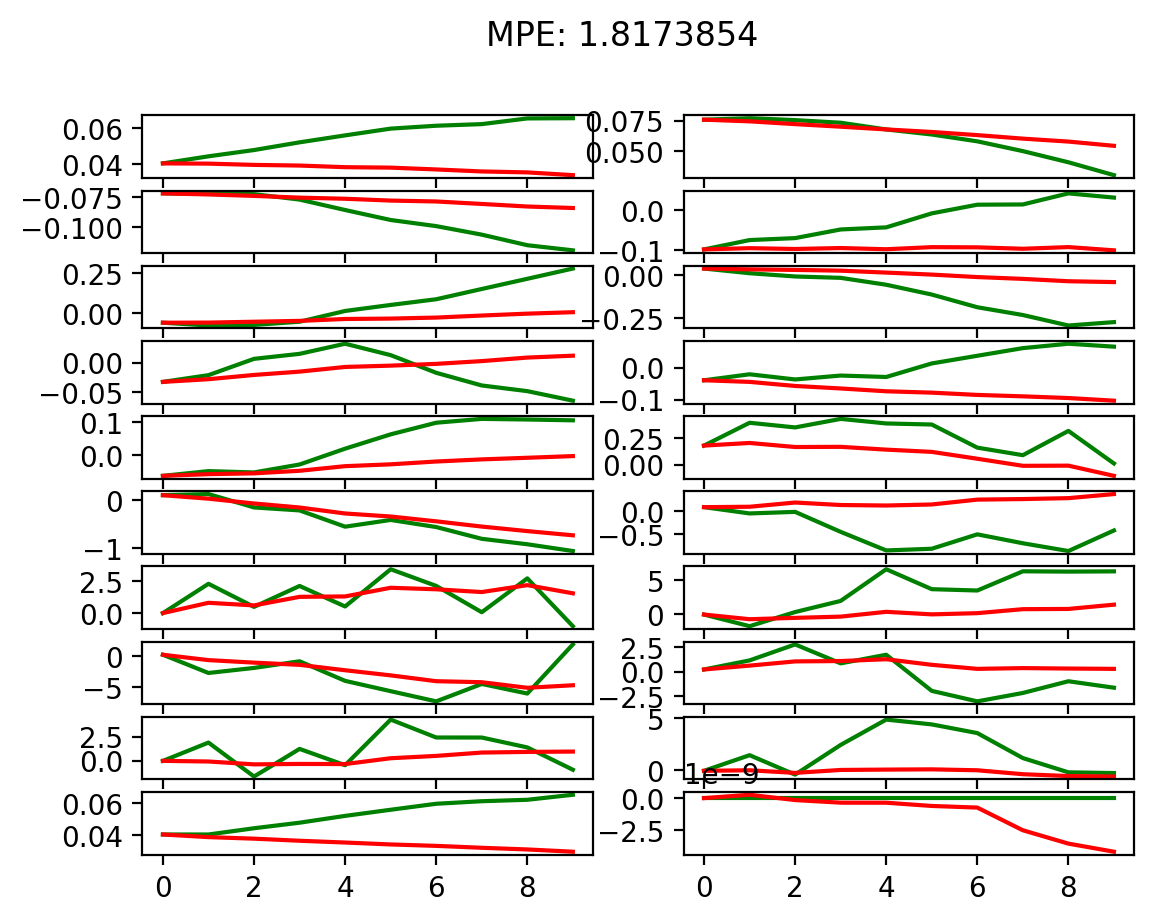
\includegraphics[width=.9\linewidth]{./hw2_q1_cheetah_n5_arch2x250_cheetah-ift6163-v0_17-02-2022_21-24-04/itr_0_predictions.png}
\caption{Experiment: \texttt{cheetah\_n5\_arch2x250}}
\end{figure}

\begin{figure}[htbp]
\centering
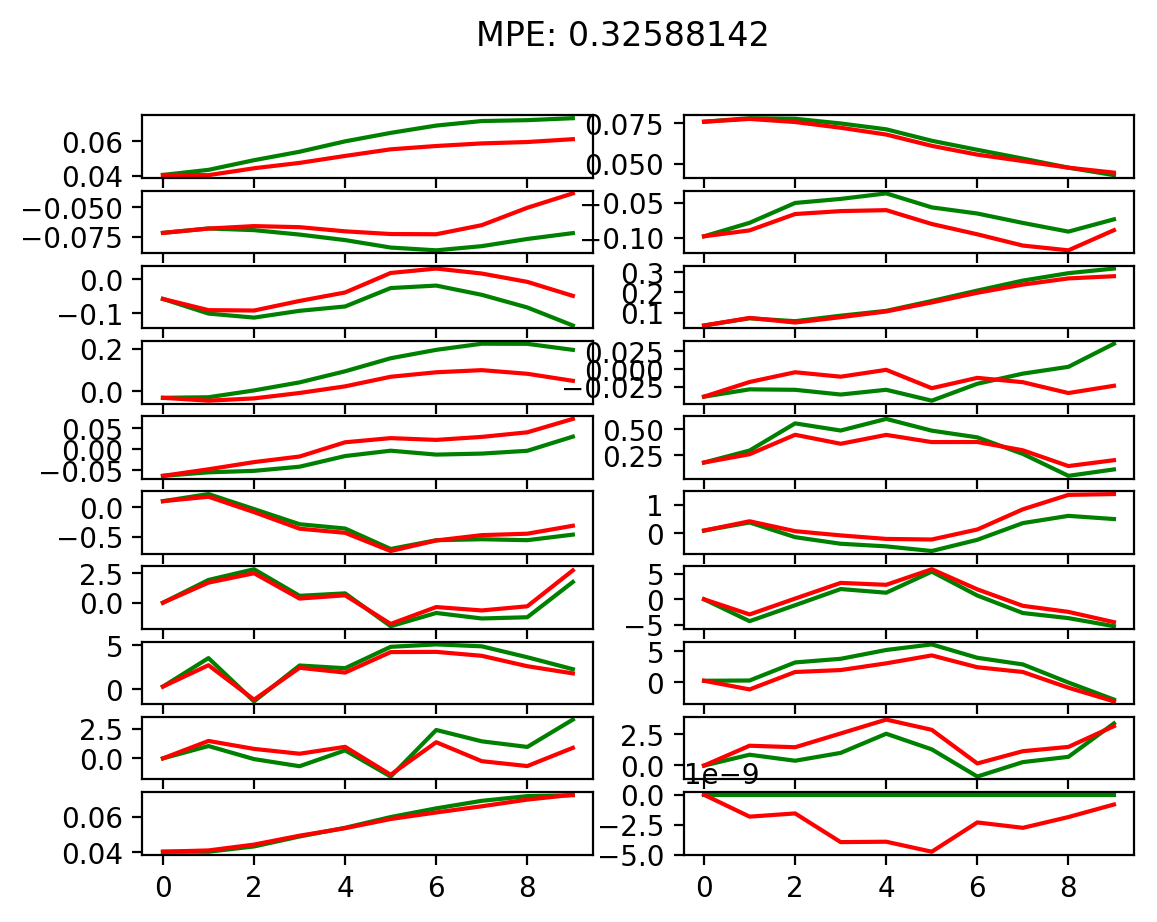
\includegraphics[width=.9\linewidth]{./hw2_q1_cheetah_n500_arch1x32_cheetah-ift6163-v0_17-02-2022_21-23-37/itr_0_predictions.png}
\caption{Experiment: \texttt{cheetah\_n500\_arch1x32}}
\end{figure}

\begin{figure}[htbp]
\centering
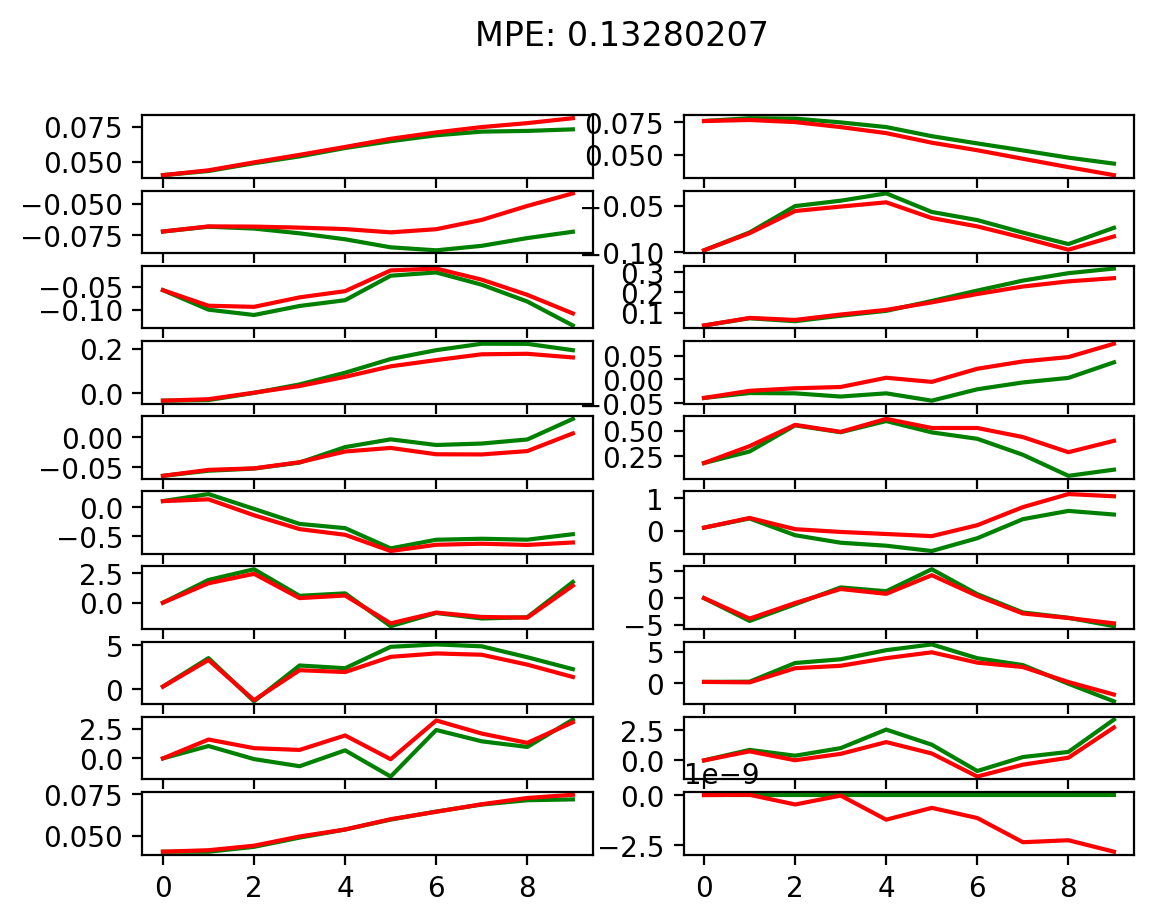
\includegraphics[width=.9\linewidth]{./hw2_q1_cheetah_n500_arch2x250_cheetah-ift6163-v0_17-02-2022_21-24-36/itr_0_predictions.png}
\caption{Experiment: \texttt{cheetah\_n500\_arch2x250}}
\end{figure}

The models corresponding to the last plot seem to be performing best. The first is trained only for a few number of iterations, i.e. 5. The second one has low network capacity, which apparently is not able to capture all the nuances of the underlying dynamics of the environment.

\clearpage

\section{Problem 2}
\label{sec:orgadd9344}

\begin{table}[htbp]
\caption{Problem 2 results}
\centering
\begin{tabular}{l|r|r}
\hline
\texttt{cheetah} & \texttt{Eval\_AverageReturn} & \texttt{Train\_AverageReturn}\\
\hline
\texttt{AverageReturn} & -32.15 & -167.19\\
\hline
\end{tabular}
\end{table}

\begin{figure}[htbp]
\centering
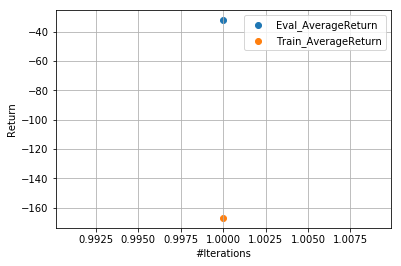
\includegraphics[width=.9\linewidth]{./q2.png}
\caption{Problem 2 plot}
\end{figure}

\clearpage

\section{Problem 3}
\label{sec:org457aaf3}
Performance plots:

\begin{figure}[htbp]
\centering
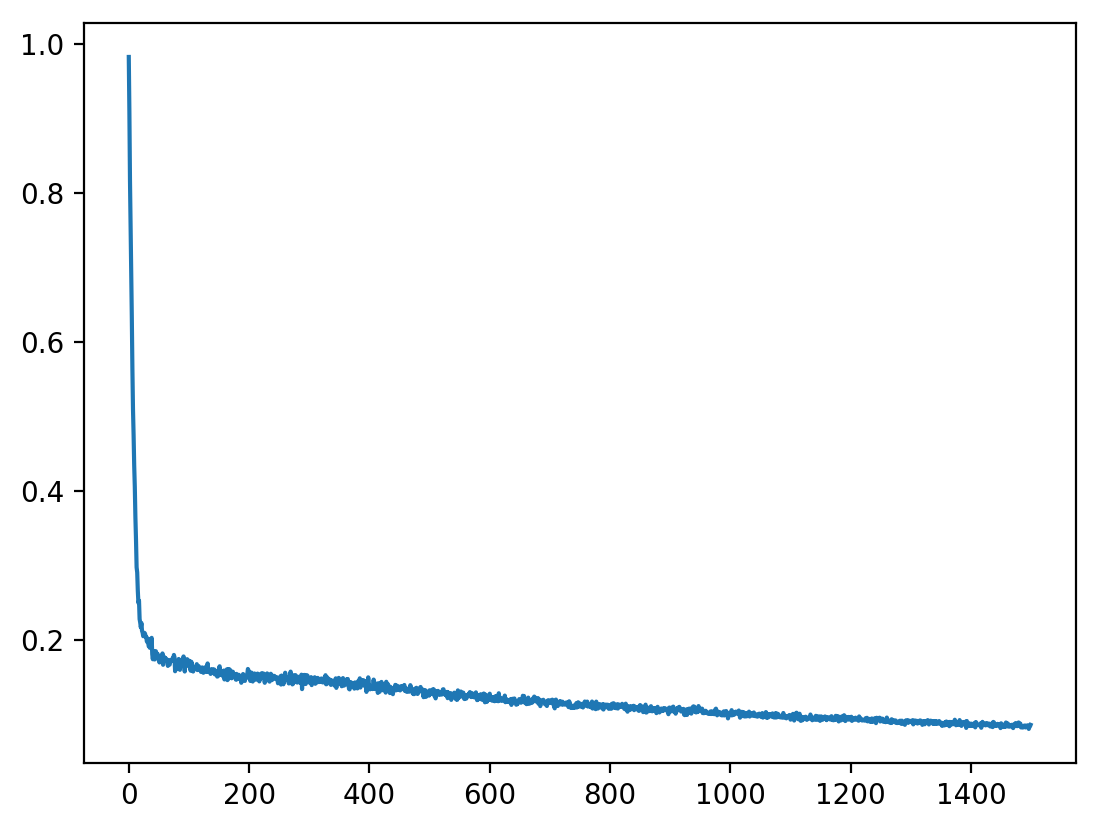
\includegraphics[width=.9\linewidth]{./hw2_q3_cheetah_cheetah-ift6163-v0_17-02-2022_22-07-54/itr_0_losses.png}
\caption{Training loss for \texttt{q3\_cheetah}}
\end{figure}

\begin{figure}[htbp]
\centering
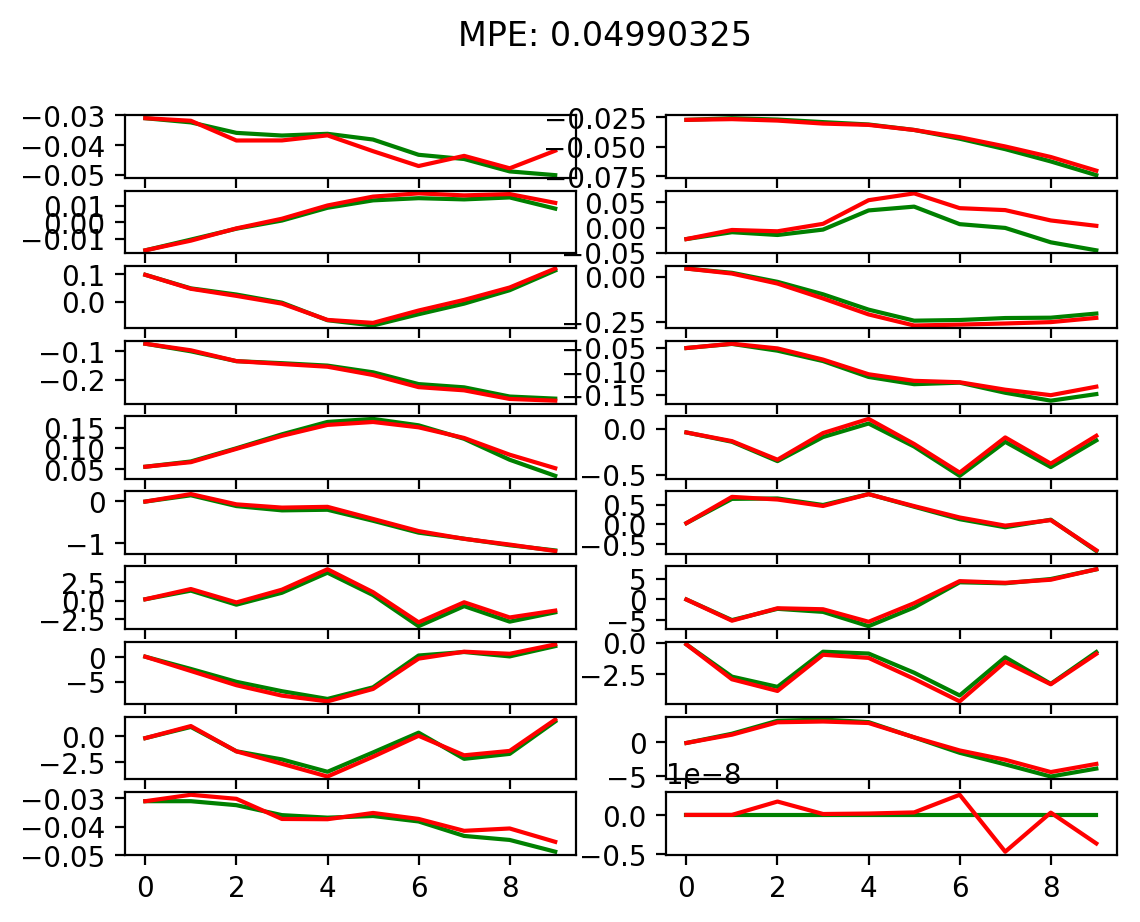
\includegraphics[width=.9\linewidth]{./hw2_q3_cheetah_cheetah-ift6163-v0_17-02-2022_22-07-54/itr_0_predictions.png}
\caption{Model errors for \texttt{q3\_cheetah}}
\end{figure}

\begin{figure}[htbp]
\centering
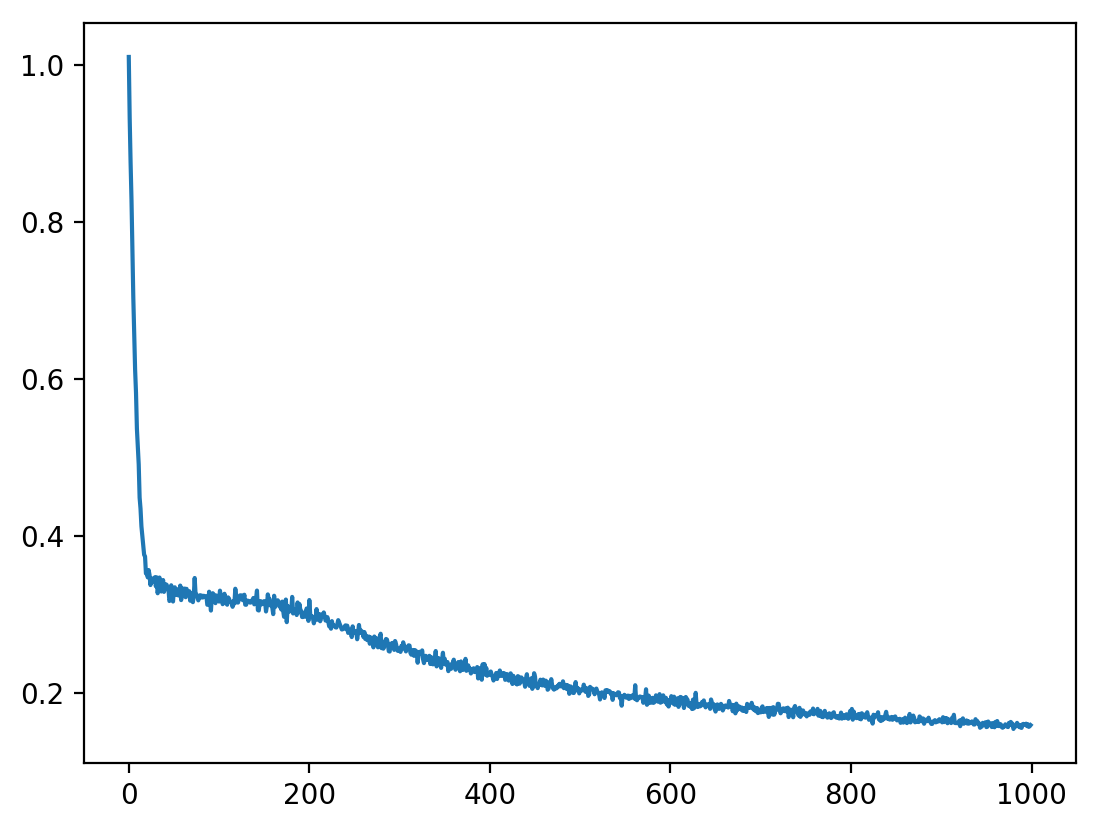
\includegraphics[width=.9\linewidth]{./hw2_q3_reacher_reacher-ift6163-v0_17-02-2022_21-58-46/itr_0_losses.png}
\caption{Training loss for \texttt{q3\_reacher}}
\end{figure}

\begin{figure}[htbp]
\centering
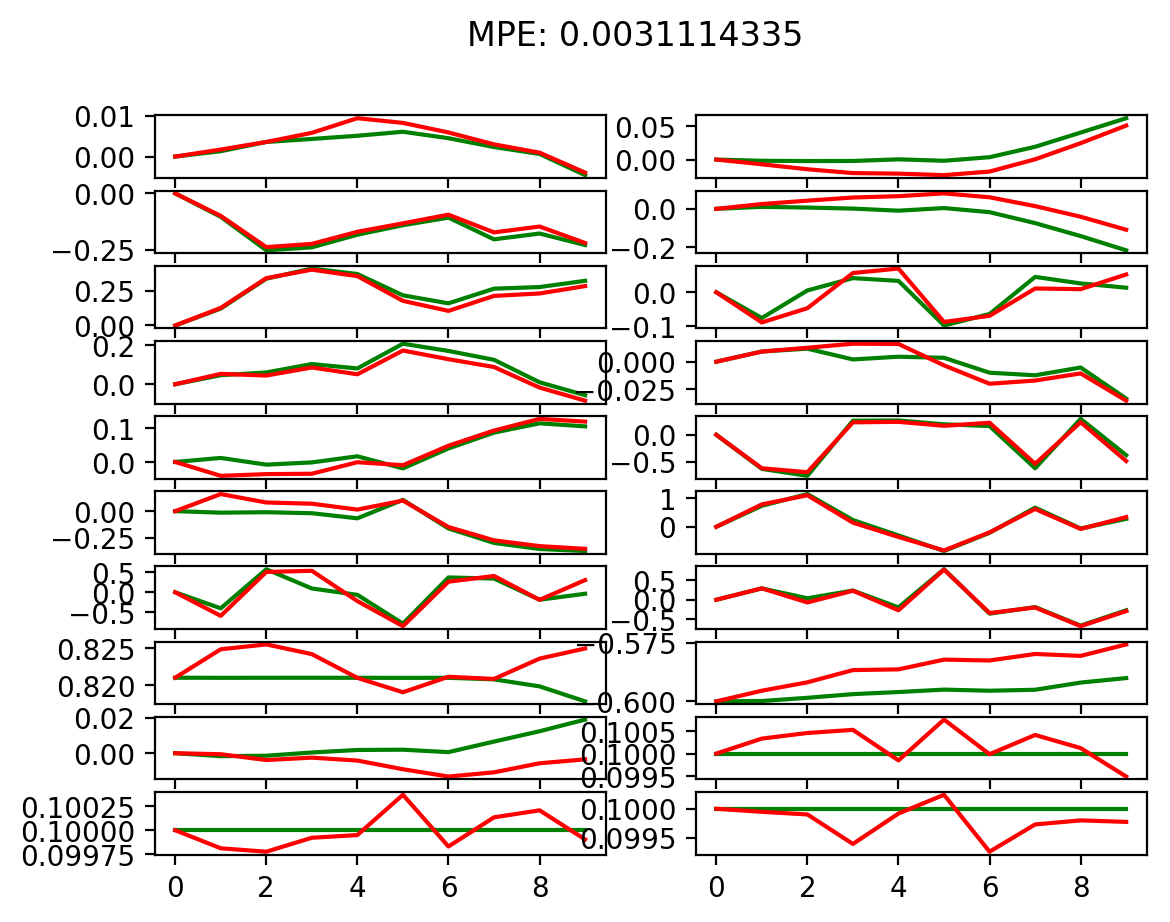
\includegraphics[width=.9\linewidth]{./hw2_q3_reacher_reacher-ift6163-v0_17-02-2022_21-58-46/itr_0_predictions.png}
\caption{Model errors for \texttt{q3\_reacher}}
\end{figure}

\begin{figure}[htbp]
\centering
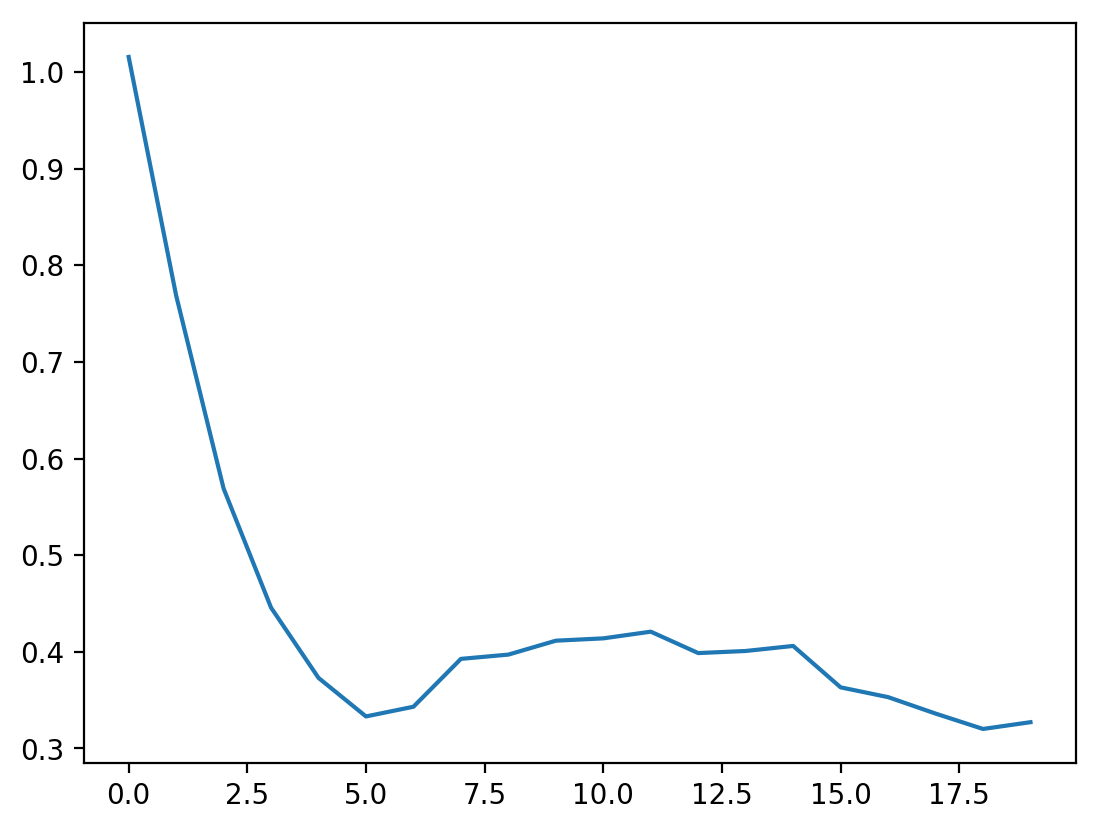
\includegraphics[width=.9\linewidth]{./hw2_q3_obstacles_obstacles-ift6163-v0_17-02-2022_21-59-34/itr_0_losses.png}
\caption{Training loss for \texttt{q3\_obstacles}}
\end{figure}

\begin{figure}[htbp]
\centering
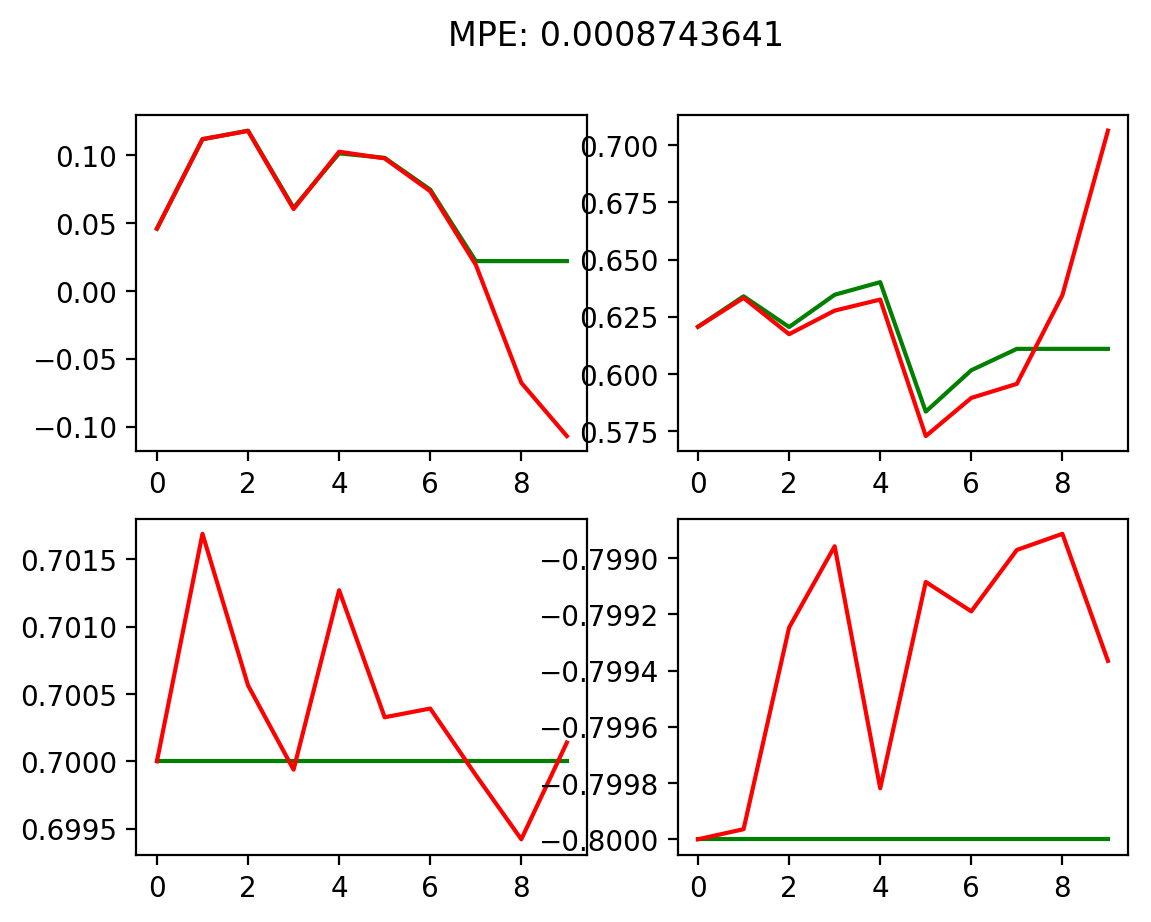
\includegraphics[width=.9\linewidth]{./hw2_q3_obstacles_obstacles-ift6163-v0_17-02-2022_21-59-34/itr_0_predictions.png}
\caption{Model errors for \texttt{q3\_obstacles}}
\end{figure}

\clearpage

\section{Problem 4}
\label{sec:orgb50809b}
\subsection{Ensembles}
\label{sec:orga8f8e7d}
\begin{figure}[htbp]
\centering
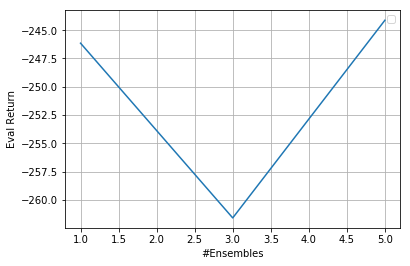
\includegraphics[width=.9\linewidth]{./ensembles.png}
\caption{Ablation with regards to the number of ensembles}
\end{figure}


\begin{figure}[htbp]
\centering
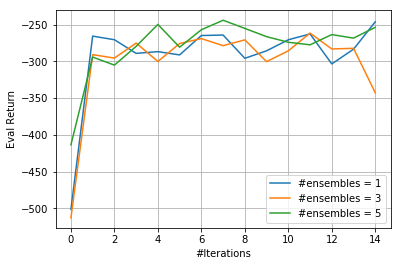
\includegraphics[width=.9\linewidth]{./ensembles_eval.png}
\caption{\texttt{Eval\_AverageReturn} with different number of ensembles}
\end{figure}

\clearpage

\subsection{MPC \# Action Sequences}
\label{sec:org823ab9c}
\begin{figure}[htbp]
\centering
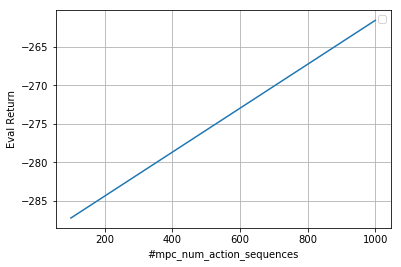
\includegraphics[width=.9\linewidth]{./numseqs.png}
\caption{Ablation with regards to the number sequence candidates}
\end{figure}

\begin{figure}[htbp]
\centering
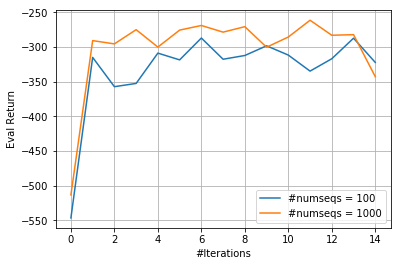
\includegraphics[width=.9\linewidth]{./numseqs_eval.png}
\caption{\texttt{Eval\_AverageReturn} with different number of sequence candidates}
\end{figure}

\clearpage

\subsection{Horizon}
\label{sec:orgf0cac6d}

\begin{figure}[htbp]
\centering
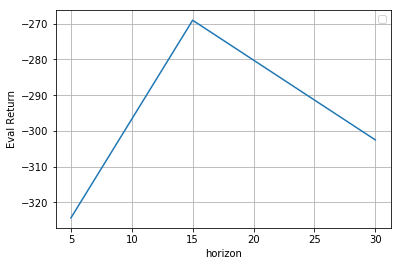
\includegraphics[width=.9\linewidth]{./horizons.png}
\caption{Ablation with regards to the planning horizon}
\end{figure}

\begin{figure}[htbp]
\centering
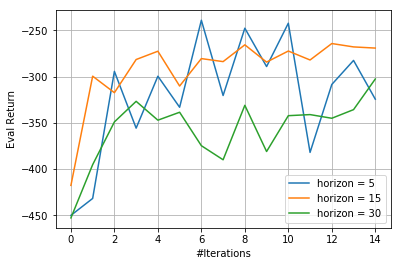
\includegraphics[width=.9\linewidth]{./horizon_eval.png}
\caption{\texttt{Eval\_AverageReturn} with different horizons.}
\end{figure}


\clearpage

\section{Problem 5}
\label{sec:org284be20}

\begin{figure}[htbp]
\centering
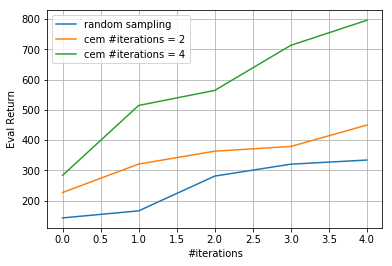
\includegraphics[width=.9\linewidth]{./cem.png}
\caption{CEM compared to random actions. CEM clearly outperforms random sampling method, since directs the search using some sort of a heuristic. Moreover, more iterations in CEM leads to more accurate results and a thorough search over the planning space.}
\end{figure}
\end{document}
